The vessel diameter is an important indicator for many vascular diseases
from the X-Ray angiogram and the precise estimation of vascular centerlines
and widths is very important for the quantitative and visualized diagnosis
of blood vessel disease. Currently the diagnosis of the vessel from the
angiograms mainly depends on doctors' naked eyes. The diagnosis results are
much affected by human factors and lead to coarse objectivity and low
accuracy.

In our approach, we combine the centerlines and the extracted vascular
structures and use the centerlines as sample bases for diameter computation.
Due to the discreteness of extracted results,  we propose a method based on
line fitting to obtain continuous diameters shown in Figure
\ref{fig:line_fitting}.

\begin{figure}
  \centering
  % Requires \usepackage{graphicx}
  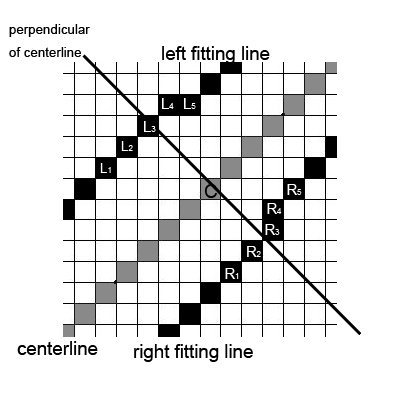
\includegraphics[width=3.0in]{line_fitting.png}\\
  \caption{Vessel Diameter Extraction}\label{fig:line_fitting}
\end{figure}

First, for specified centerline point $C(i,j)$ , we get two adjacent
neighbours on both its left and right side. Using this five points including
the point $C(i,j)$, we get the line $L_{c}$ crossing the centerline point.
Then we can achieve the perpendicular line's slope at point $C(i,j)$ and
compute its intersection point with the vascular structures contour $L_{3}$
and $R_{3}$. With these two points, we get the forward and backwards two
points of the contour. Then, we get the left intersection group $L=(L_{1},
L_{2}, L_{3}, L_{4}, L_{5})$ and the right $R=(R_{1}, R_{2}, R_{3}, R_{4},
R_{5})$ and the fitting lines $L_{l}$ and $L_{r}$ using the point groups. At
last, we obtain the intersection of $C_{L}(x_{l}, y_{l})$($L_{c}$ and
$L_{l}$) and $C_{R}(x_{r}, y_{r})$($L_{c}$ and $L_{r}$). We use the distance
$D=\sqrt{(x_{l}-x_{r})^2 + (y_{l}-y_{r})^2}$ as the vessel diameter at the
right position $C(i,j)$.

Using this method, we extract the diameters of Figure
\ref{fig:lineseg_trace},
%and the results are shown in Figure
%\ref{fig:diameter_extraction},
which are continuous and with slight
waving values.

%%\begin{figure}
%%  \centering
%%  % Requires \usepackage{graphicx}
%%  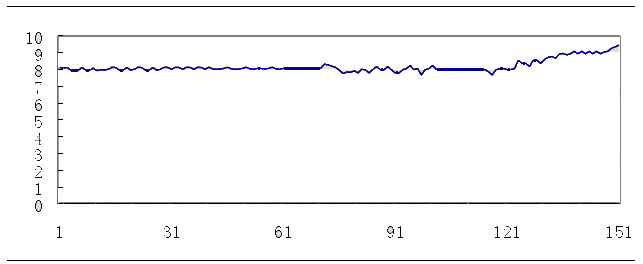
\includegraphics[width=3.0in]{diameter_extraction.png}\\
%%  \caption{Vessel Diameter Extraction Results}\label{fig:diameter_extraction}
%% \end{figure}
